% -*- compile-command: "pdflatex cyd-2015-02-26.tex"; -*-

\documentclass[a4paper,12pt]{article}
\usepackage[utf8]{inputenc}
\usepackage[swedish]{babel}
\usepackage{enumerate}
\usepackage{hyperref}
\usepackage{pdfpages}
\usepackage{graphicx}

\begin{document}
\section{CYD-poolens styrelsemöte 2016-02-15}

\def\arraystretch{1.3}
\begin{tabular*}{\textwidth}{@{\extracolsep{\fill} }l c r}
Närvarande & Ämbete & Funktion \\
\hline\\[-0.4cm]
Kristina Arkad & Teknisk chef ISY & Ledamot\\
Christian Luckey & Systemadministratör & Ledamot\\
Hans-Filip Elo & Systemadministratör & Ordförande\\
Martin Estgren & Systemadministratör & Sekreterare\\
Tea Nygren & Utbildningsledare DM-nämnden & Justerare\\ 
Erik Sköld & Webbmaster, Y-sektionen & Ledamot\\
Michael Sörsäter & Sekreterare D-sektionen & Ledamot\\
Patrik Sletmo & D-LAN, D-Group, D-sektionen & Adjungant\\
Victor Karlsson Sehlin & Webbmaster, D-sektionen & Adjungant\\[2cm]
\end{tabular*}

\begin{enumerate}
\item Mötet öppnande.
\item Eventuella adjungeringar till mötet.
\item Hans-Filip valdes till ordförande.
\item Martin Estgren valdes till sekreterare samt Tea Nygren och Hans-Filip till justerare.
\item Verksamhetsberättelse.
\begin{itemize}
\item Rekrytering - vi har rekryterat Martin.
\item Nya siter: D-LAN och Valla Saucer Rennen.
\item Automatiserad SSL-labs scanning mot alla CYD-siter.
\item Automatiserade HTTPs-certifikat från Let's encrypt.
\item Nya UPS-batterier.
\item Klimatsensor uppsatt i CYD. CYD-poolen har nu data att presentera rörande luftkvalitén.
\end{itemize}
\newpage
\item Detta ligger i CYDs pipeline just nu:
\begin{itemize}
\item Linux på desktopen.
\item Mailserver för linkdagarna fortfarande i pipe:n.
\item Redundanta switchar.
\end{itemize}
\item Återkoppling: Luftkvalitén i CYD.
\begin{itemize}
\item Christian Luckey visar fina grafer över CO2 halt (se appendix A).
\item CYD-Administratörerna ålägger sig att skicka vidare data om CO2 halt till akademiska hus.
\item Prata med arbetsmiljöombud för D och Y sektionen och skicka dem data gällande CO2 halt.
\end{itemize}
\item Läsning av utkast för SLA.
\begin{itemize}
\item Utkast till SLA presenteras av Hans-Filip och diskuteras. 
\item Styrelsen förhåller sig välvilliga till den presenterade strukturen men vill ha återkoppling från studentorganisationerna. 
\item CYD-Administratörerna ålägger sig att skicka ut SLA-utkast till berörda studentorganisationerna för återkoppling.
\end{itemize}
\item Övriga frågor.
\item Nästa Sammanträde sätts preliminärt till 2016-09-12
\item Mötet avslutas.
\end{enumerate}

\vspace{2cm}
\noindent
Justeras:
~\\
~\\
~\\
~\\
\noindent\begin{tabular}{ll}
\makebox[0.5\textwidth]{\hrulefill} & \makebox[0.5\textwidth]{\hrulefill}\\
Namn & Datum\\[1.5cm]
\makebox[0.5\textwidth]{\hrulefill} & \makebox[0.5\textwidth]{\hrulefill}\\
Namn & Datum\\
\end{tabular}
~\\
Appendix A: Fin graf
~\\
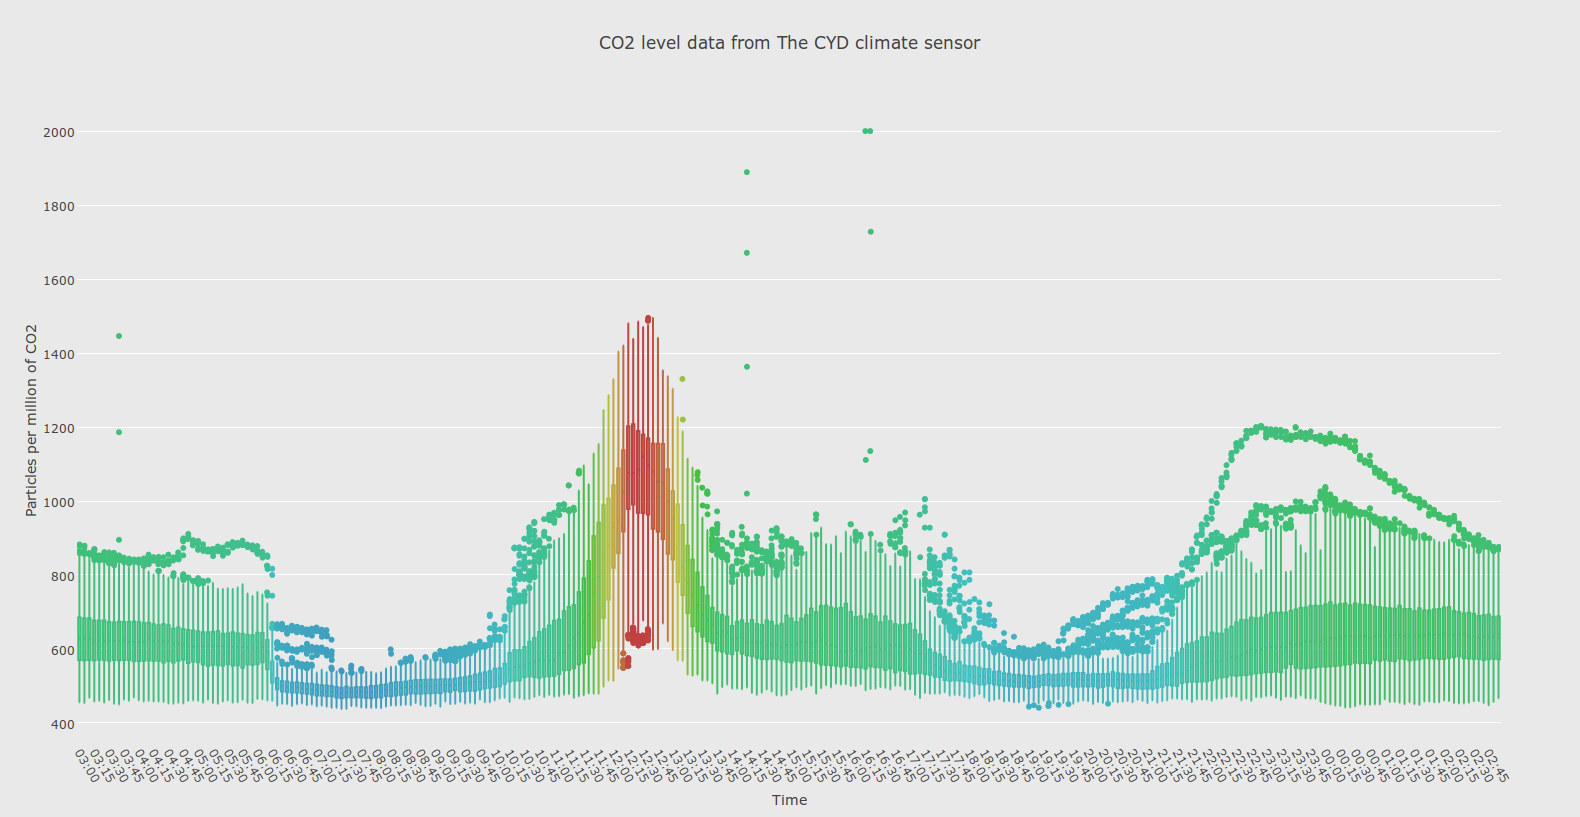
\includegraphics[height=\textwidth, width=\textheight, angle=90]{2016-02-15-appendix-a.png}

% ------
\end{document}
